%%%%%%%%%%%%%%%%%%%%%%%%%%%%%%%
%%%%%%%%%%%%%%%%%%%%%%%%%%%%%%%
\chapter{Methods\label{ch:methods}}
%%%%%%%%%%%%%%%%%%%%%%%%%%%%%%%
The system identification of ship dynamics can be simplified into parameter identification if parameterized physical models can be assumed. Parameter Identification Techniques (PIT) for roll motion an manoeuvring is presented in \ref{sec:PIT_roll} and \ref{sec:PIT_VMM}. The system identification can be performed by selecting the best model from a collection of candidate models.

\section{Roll damping Parameter Identification} \label{sec:PIT_roll}
\noindent The PIT can be applied to identify the roll damping parameters ($B_1$, $B_2$, $B_3$) and stiffness parameters ($C_1$, $C_3$, $C_5$) in the parameterized roll motion models in Eq.\ref{eq:roll_decay_equation_himeno_linear}, Eq.\ref{eq:roll_decay_equation_himeno_quadratic_b} and Eq.\ref{eq:roll_decay_equation_cubic}. These equations do not have unique solutions, considering that the whole equations can be multiplied by an arbitrary factor to obtain new valid solutions. The inertia is therefore excluded, to obtain unique solutions. This is achieved by normalizing the equations by the total roll inertia $A_{44}$.
The normalized damping and stiffness parameters identified by a PIT can be expressed in dimensional units by multiplication with the normalization factor $A_{44}$. If $A_{44}$ is not known before hand, it can be calculated using Eq.\ref{eq:A_44_eq} \cite{piehl_ship_2016}, assuming that the meta center height $GM$ is known.
\begin{equation} \label{eq:A_44_eq}
A_{44} = \frac{GM g m}{\omega_{0}^{2}}
\end{equation}

\noindent The frequency $\omega_0$ can be obtained with Fast Fourier Transform (FFT) of the roll signal. 

Two different PIT methods have been investigated: the ``derivation approach'' (referred to as PIT in \parencite{imo_1200_2006}) and the ``integration approach'' which is similar to what \parencite{soder_assessment_2019} used. In the derivation approach the first and second roll time derivatives are calculated numerically so that the parameters in the models are the only unknowns. A least squares fit is applied on the roll motion equation to identify any parameter, including nonlinear or frequency parameter. In the integration approach, the parameters are found by solving a nonlinear problem using the least-square method. This approach requires that an ordinary differential equation to be solved for many estimated sets of parameters until the solution converges.

\section{Roll damping model}
A serial grey-box model for ship roll damping (see Fig.\ref{fig:greyrolldamping}) is developed in Paper \ref{pap:rolldamping}. Simplified Ikeda's (SI) method \cite{kawahara_simple_2011} is used as the white box model, which is combined with a following black-box correction model.

\begin{figure}[H]
    
    \centering
    \begin{tikzpicture}[node distance=2cm]
    \node (white-box) [white-box] {Simplified Ikeda};
    \node (B_BK) [io, right of=white-box, xshift=0.90cm, yshift=1.5cm] {$\hat{B_{BK}}$};
    \node (B_E) [io, right of=white-box, xshift=0.75cm, yshift=0.75cm] {$\hat{B_{E}}$};
    \node (B_F) [io, right of=white-box, xshift=0.75cm, yshift=0cm] {$\hat{B_{F}}$};
    \node (B_L) [io, right of=white-box, xshift=0.75cm, yshift=-0.75cm] {$\hat{B_{L}}$};
    \node (B_W) [io, right of=white-box, xshift=0.75cm, yshift=-1.5cm] {$\hat{B_{W}}$};
    
    
    \node (black-box) [black-box, right of=B_F, xshift=0.75cm] {Black-box};
    \draw [arrow] (white-box) -- (B_BK);
    \draw [arrow] (white-box) -- (B_E);
    \draw [arrow] (white-box) -- (B_F);
    \draw [arrow] (white-box) -- (B_L);
    \draw [arrow] (white-box) -- (B_W);
    
    \draw [arrow] (B_BK) -- (black-box);
    \draw [arrow] (B_E)  -- (black-box);
    \draw [arrow] (B_F)  -- (black-box);
    \draw [arrow] (B_L)  -- (black-box);
    \draw [arrow] (B_W)  -- (black-box);
    
    
    \node (B) [io, right of=black-box, xshift=0.75cm, yshift=0cm] {$B$};
    \draw [arrow] (black-box)  -- (B);
    
    \end{tikzpicture}
    \caption{Grey-box model to predict roll damping}
    \label{fig:greyrolldamping}
\end{figure}

\noindent A roll damping dataset is used to train the black-box part of the grey-box model.
250 roll decay tests assembled from the Maritime Dynamics Laboratory at SSPA Sweden AB (\href{www.sspa.se}{www.sspa.se}) are used to build the dataset. The roll damping parameters are found by applying a PIT (see Section \ref{sec:PIT_roll}) on the parameterized roll motion models (see Section \ref{sec:roll}).

\section{VMM Parameter Identification} \label{sec:PIT_VMM}
The proposed PIT is summarized in Fig.\ref{fig:greyvmm}. In this procedure, a VMM is used to solve the reversed manoeuvring problem, such as predicting unknown forces from known manoeuvring model test data. The hydrodynamic derivatives in the VMM can be identified with regression of the force polynomials on forces predicted with inverse dynamics.
The measurement noise needs to be removed if the regression of hydrodynamic derivatives in the VMM should work well. This is conducted by a Extended Kalman Filter (EKF) and Rauch Tung Striebel (RTS) smoother (see section \ref{sec:datacleaning}). The EKF requires an accurate VMM as the predictor.
Therefore the accurate VMM is both the input and output of the PIT. The system model VMM in the EKF is guessed to solve this dilemma. A linear VMM with hydrodynamic derivatives estimated with semi-empirical formulas is used as the initial guess. Once the regressed VMM has been obtained, the PIT can be rerun using the regressed VMM as the system model in the EKF, to obtain an even better VMM. This procedure, indicated by the dashed arrow in Fig.\ref{fig:greyvmm}, can be repeated several times for improved accuracy. Using semi-empirical formulas for the initially guessed VMM adds prior knowledge about the ship dynamics to the regression. An example with simulation results from the steps in the iterative EKF is shown in \hyperref[\detokenize{01.01_method:iterations}]{Fig.\@\ref{\detokenize{01.01_method:iterations}}}.

\begin{figure}[H]
    
    \centering
    \begin{tikzpicture}[node distance=2cm]
    \node (data) [io, above of=white-box, xshift=1cm, yshift=1.5cm] {Model test data};
    
    \node (EKF) [process, right of=data, xshift=2.5cm, yshift=0cm] {EFK + RTS};
    \node (predictor) [process, right of=EKF, xshift=1.5cm, yshift=0cm]{Predictor};
    \node (VMM) [io, right of=predictor, xshift=1.5cm, yshift=0cm] {VMM initial};
    
    \node (data_clean) [io, below of=EKF, xshift=0cm, yshift=0.0cm] {\(x,\dot{x},\ddot{x}, \delta, thrust\)};
    
    \node (white-box) [white-box] {Inverse dynamics};
    \node (X_D) [io, right of=white-box, xshift=0.90cm, yshift=1cm]{\(X_D\)};
    \node (Y_D) [io, right of=white-box, xshift=0.90cm, yshift=0cm]{\(Y_D\)};
    \node (N_D) [io, right of=white-box, xshift=0.90cm, yshift=-1cm]{\(N_D\)};
    
    \node (black-box) [black-box, right of=B_F, xshift=0.75cm] {Regression};
    
    \node (coefficients) [io, right of=black-box, xshift=1.5cm, yshift=0cm] {VMM$\left(Y_{uv},N_{\delta},...\right)$};
    
    
    \draw [arrow] (data) -- (EKF);
    \draw [arrow] (predictor) -- (EKF);
    \draw [arrow] (VMM) -- (predictor);
    \draw [arrow] (EKF) -- (data_clean);
    
    \draw [arrow] (data_clean) -| (white-box);
    \draw [arrow] (data_clean) -- (black-box);
    
    \draw [arrow] (white-box) -- (X_D);
    \draw [arrow] (white-box) -- (Y_D);
    \draw [arrow] (white-box) -- (N_D);
    
    \draw [arrow, shorten >=0.5cm] (X_D) -- (black-box);
    \draw [arrow, shorten >=0.2cm] (Y_D)  -- (black-box);
    \draw [arrow, shorten >=0.5cm] (N_D)  -- (black-box);
    
    \draw [arrow] (black-box)  -- (coefficients);
    \draw [arrow, dashed] (coefficients)  -- (predictor);
    
    \end{tikzpicture}
    \caption{Grey-box model to predict the VMM hydrodynamic derivatives}
    \label{fig:greyvmm}
\end{figure}

\begin{figure}[h]
    \centering
    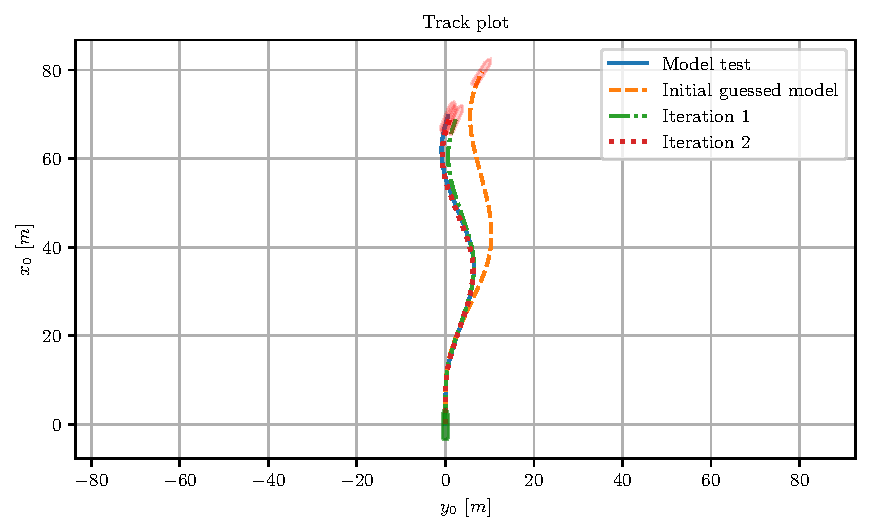
\includegraphics[width=\textwidth]{kappa/images/0.pdf}
    \caption{Simulation with: initial model, first and second iteration of the PIT}
    \label{\detokenize{01.01_method:iterations}}
\end{figure}

\subsection{Inverse dynamics and regression}
\label{\detokenize{03.01_inverse_dynamics:inverse-dynamics-and-regression}}\label{\detokenize{03.01_inverse_dynamics::doc}}
\sphinxAtStartPar
Each manoeuvring model has some hydrodynamic functions \(X_D(u,v,r,\delta,thrust)\), \(Y_D(u,v,r,\delta,thrust)\), \(N_D(u,v,r,\delta,thrust)\) that are defined as polynomials. The hydrodynamic derivatives in these polynomials can be identified with force regression of measured forces and moments. The measured forces and moments are usually taken from Captive Model Tests (CMT), Planar Motion Mechanism (PMM) tests or Virtual Captive Tests (VCT). When the ship is free in all degrees of freedom, as in the present model tests, only
motions are recorded however. Hence, forces and moments causing ship motions need to be estimated by
solving the inverse dynamics problem.
The inverse dynamics is solved by restructuring the system equation (\autoref{equation:02.01_VMMs:eqqsystem}) to get the hydrodynamics functions on the left-hand side. If the mass and inertia of the ship including added masses: \(X_{\dot{u}}\), \(Y_{\dot{v}}\), \(Y_{\dot{r}}\), \(N_{\dot{v}}\) and \(N_{\dot{r}}\), are known, the forces in Prime system can be calculated using \autoref{equation:03.01_inverse_dynamics:eqxd}, \autoref{equation:03.01_inverse_dynamics:eqyd} and \autoref{equation:03.01_inverse_dynamics:eqnd}.
The Ordinary Least Square (OLS) method regresses the hydrodynamic derivatives. 
\begin{equation}\label{equation:03.01_inverse_dynamics:eqxd}
\begin{split}\displaystyle \operatorname{X_{D}'}{\left(u',v',r',\delta,thrust' \right)} = - X_{\dot{u}}' \dot{u}' + \dot{u}' m' - m' r'^{2} x_{G}' - m' r' v'\end{split}
\end{equation}\begin{equation}\label{equation:03.01_inverse_dynamics:eqyd}
\begin{split}\displaystyle \operatorname{Y_{D}'}{\left(u',v',r',\delta,thrust' \right)} = - Y_{\dot{r}}' \dot{r}' - Y_{\dot{v}}' \dot{v}' + \dot{r}' m' x_{G}' + \dot{v}' m' + m' r' u'\end{split}
\end{equation}\begin{equation}\label{equation:03.01_inverse_dynamics:eqnd}
\begin{split}\displaystyle \operatorname{N_{D}'}{\left(u',v',r',\delta,thrust' \right)} = I_{z}' \dot{r}' - N_{\dot{r}}' \dot{r}' - N_{\dot{v}}' \dot{v}' + \dot{v}' m' x_{G}' + m' r' u' x_{G}'\end{split}
\end{equation}
\sphinxAtStartPar
An example of forces calculated with inverse dynamics from motions in a turning circle test can be seen in \hyperref[\detokenize{03.01_inverse_dynamics:fig-inverse}]{Fig.\@ \ref{\detokenize{03.01_inverse_dynamics:fig-inverse}}}. The forces have been converted to SI units.

\begin{figure}[H]
    \centering
    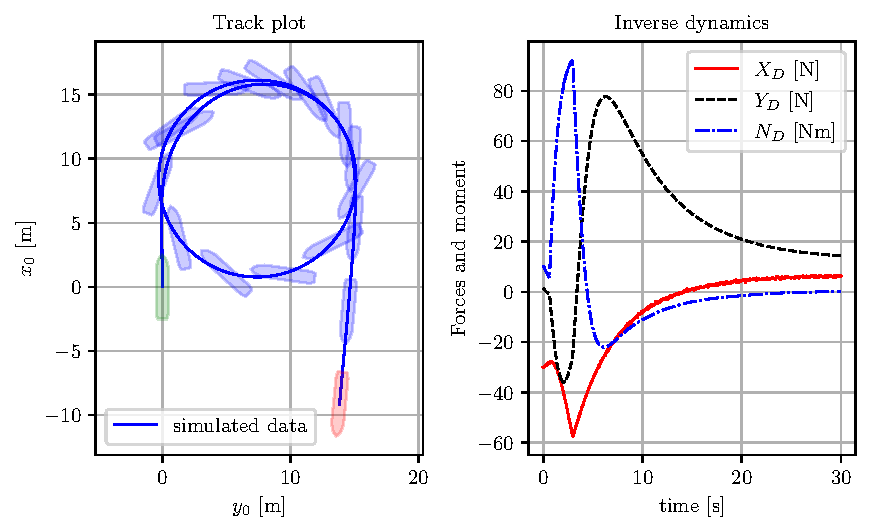
\includegraphics[width=\textwidth]{kappa/images/1.pdf}
    \caption{Example of forces and moments calculated with inverse dynamics on data from a turning circle test.}
    \label{\detokenize{03.01_inverse_dynamics:fig-inverse}}
\end{figure}

\subsection{Data cleaning}
\label{sec:datacleaning}
It is possible to do an exact parameter identification on perfect (simulated) data with no noise (see Paper \ref{pap:pit}). However, such data from physical experiments does not exist in reality. The measured data will always contain process noise and measurement noise. In order to mitigate this, the data is preprocessed using the EKF and RTS smoother which are both presented below.

EKF is an extension of the Kalman Filter (KF) to work on nonlinear systems such as the VMMs. The basic idea is that noise can be disregarded if it does not make sense from a physical point of view. If noisy measurement data were perfectly correct, this would mean that the ship has many vibrations that must have originated from tremendous forces, considering the large mass of the ship. The prior understanding of the dynamics suggests that these forces are not present. Therefore, the noise should be considered as measurement noise and should be removed. Low-pass filtering is a common way to remove noise, where motions above some cut-off frequencies are regarded as unphysical measurement noise. The problem with low-pass filter is that it is hard to know what cut-off frequency to choose, either too low: removing part of the signal, or too high: keeping some unfiltered measurement noise in the data. The Kalman filter has a system model that continuously estimates the system’s state that runs in parallel with the measurement data. The filter estimates the current state as a combination of the measurement data and the system model estimate based on belief in the data and the model. If the data has low noise, the estimate turns toward that data. Conversely, if the model gives very good predictions, then that estimate turns towards the model.
The system’s inverse dynamics require the entire states, including positions, velocities, and accelerations, to be known. Only positions are known from the measurements, which means that velocities and accelerations are hidden states that the EKF should estimate.

The EKF is recursive and can be run online, continuously making new estimates as new measurements arrive. The EKF uses passed measurements to estimate states in the near future. This property is helpful for online applications such as  autopilots or autonomous ships. This restriction is  unnecessary for the PIT on already existing data where a whole time series of existing measurements are available. The fact that both past and future data are known can be used to improve the filter. An EKF filter can include future time steps by adding a smoother after the filter. The PIT uses a Rauch Tung Striebel (RTS) smoother \cite{rauch_maximum_1965}, which is an algorithm that runs the EKF backward to also account for future time steps.


